\documentclass[../main.tex]{subfiles}
\graphicspath{{\subfix{../images/}}}
\begin{document}
\section*{Term 1 Week 8}
\begin{enumerate}
    \item 
    Parabola gradient:\\
    \(\frac{dy}{dx}=2x\)\\
    Therefore, the gradient of the normal is \(-\frac{1}{2x}\).\\

    The circle is in the form \(x^2+(y+b)^2=1\)\\
    Differentiating implicitly to get the gradient:\\
    \(2x+2(y+b)\frac{dy}{dx}=0\)\\
    \(\frac{dy}{dx}=-\frac{2x}{2(y+b)}=-\frac{x}{y+b}\)\\

    At the point of intersection \((x,y)\) we know these are equal:\\
    \(-\frac{x}{y+b}=-\frac{1}{2x}\)\\
    \(2x^2=y+b\)\\

    Substituting in \(y=x^2\), we get \(2x^2=x^2+b\)\\
    \(x^2=b\)\\
    \(x=\pm \sqrt{b}\)\\
    \(y=b\)\\

    Points of intersection are \((-\sqrt{b},b)\) and \((\sqrt{b}, b)\)\\
    Substitute into the circle equation:\\
    \((\sqrt{b})^2+(b+b)^2=1\)\\
    \(b+4b^2=1\)\\
    \(4b^2+b-1=0\)\\
    Solving for b: \(b=\frac{-1\pm \sqrt{17}}{8}\)\\
    
    Since the circle has been moved down, it must be positive, therefore \(b=\frac{-1+ \sqrt{17}}{8}=0.39\)\\

    \item 
    Since 18 is a factor 90, we can rewrite this as:\\
    \(5\theta=90\\
    2\theta + 3\theta=90\\
    2\theta=90-3\theta\)\\

    We then take sine of both sides and use compound angle rules to simplify:\\
    \(\sin{(2\theta)}=\sin{(90-3\theta)}\\
    2\sin{(\theta)}\cos{(\theta)}=\sin{(90)}\cos{(3\theta)}-\cos{(90)}\sin{(3\theta)}\\
    2\sin{(\theta)}\cos{(\theta)}=\cos{(3\theta)}\\
    2\sin{(\theta)}\cos{(\theta)}=\cos{(2\theta+ \theta)}\\
    2\sin{(\theta)}\cos{(\theta)}=\cos{(2\theta)\cos{(\theta)}-\sin{(2\theta)}\sin{(\theta)}}\\
    2\sin{(\theta)}\cos{(\theta)}=(1-2\sin^2(\theta))\cos{(\theta)}-2\sin^2(\theta)\cos{(\theta)}
    \)\\

    Divide through by \(\cos(\theta)\):\\
    \(2\sin{(\theta)}=1-2\sin^2(\theta)-2\sin^2(\theta)\\
    2\sin(\theta)=1-4\sin^2(\theta)\\
    4\sin^2(\theta)+2\sin(\theta)-1=0\)\\

    Solving the quadratic:\\
    \(\sin(\theta)=\frac{-2\pm \sqrt{20}}{8}\\
    \sin(\theta)=\frac{-2\pm 2\sqrt{5}}{8}\\
    \sin(\theta)=\frac{-1\pm \sqrt{5}}{4}\\
    \)

    Since we are finding \(\sin(18)\), which we know is positive (from our knowledge of the graph), \(\sin(18)=\frac{-1+\sqrt{5}}{4}\)\\

    There is an alternative, geometric, approach. Start by drawing an isosceles triangle with angles of 36, 72 and 72. Long sides are x and base is 1.
    \begin{figure}[H]
        \centering
        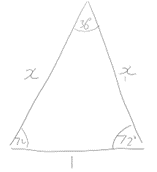
\includegraphics[width=0.2\linewidth]{images/t1w8q2_a1.png}
    \end{figure}
    Bisect one of the base angles, creating a new, smaller, triangle which is also isosceles:
    \begin{figure}[H]
        \centering
        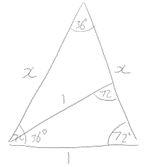
\includegraphics[width=0.25\linewidth]{images/t1w8q2_a2.png}
    \end{figure}
    This creates another isosceles triangle above it, with angles 108, 36 and 36. Therefore the sides are 1, 1 and \(x\). This means the first small triangle has a base of \(x-1\).
    \begin{figure}[H]
        \centering
        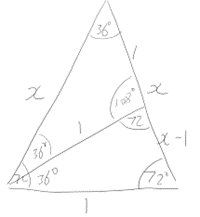
\includegraphics[width=0.25\linewidth]{images/t1w8q2_a3.png}
    \end{figure}
    Using ratios:\\
    \(\frac{x}{1}=\frac{1}{x-1}\\
    x^2-x=1\\
    x^2-x-1=0\\
    x=\frac{1+\sqrt{5}}{2}\)\\
    Finally, to get \(\sin(18)\), we can just substitute the x value in and cut the large triangle in half:
    \begin{figure}[H]
        \centering
        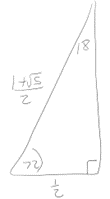
\includegraphics[width=0.15\linewidth]{images/t1w8q2_a4.png}
    \end{figure}
    Therefore, \(\sin(18)=\frac{O}{H}=\frac{\frac{1}{2}}{\frac{1+\sqrt{5}}{2}}=\frac{1}{1+\sqrt{5}}=\frac{\sqrt{5}-1}{4}\)\\
    
    \item 
    Nice solution (thanks to Aaron Moore for this):\\
    We know that the angle of the line passing through the centres of the circle is \(\frac{\pi}{8}\).
    \begin{figure}[H]
        \centering
        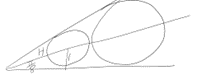
\includegraphics[width=0.25\linewidth]{images/t1w8q3_ans6.png}
    \end{figure}
    Looking at the small triangle, we know that \(\sin{\frac{\pi}{8}}=\frac{1}{H}\), therefore the hypotenuse \(H=\frac{1}{\sin{\frac{\pi}{8}}}\)\\

    The ratio of side lengths is the same for the next triangle formed at the centre of the next circle. The hypotenuse of that is \(H+1+R\):
    \begin{figure}[H]
        \centering
        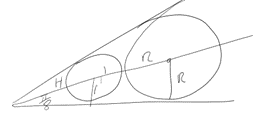
\includegraphics[width=0.25\linewidth]{images/t1w8q3_ans7.png}
    \end{figure}
    Therefore, \(\sin{\frac{\pi}{8}}=\frac{R}{\frac{1}{\sin{\frac{\pi}{8}}}+1+R}\)\\

    Rearranging:\\
    \(1+\sin{\frac{\pi}{8}}+R\sin{\frac{\pi}{8}}=R\)\\

    \(R-R\sin{\frac{\pi}{8}}=1+\sin{\frac{\pi}{8}}\)\\

    \(R(1-\sin{\frac{\pi}{8}})=1+\sin{\frac{\pi}{8}}\)\\

    \(R=\frac{1+\sin{\frac{\pi}{8}}}{1-\sin{\frac{\pi}{8}}}=2.24\)\\

    Since area = \(\pi r^2\), the larger circle is \(2.24^2=5.02\) times bigger.\\
    
    \textit{And now my algebra-heavy approach:}\\
    First, we find the line running through the centres of the circles.
    \begin{figure}[H]
        \centering
        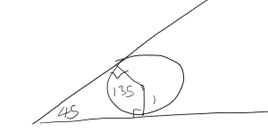
\includegraphics[width=0.25\linewidth]{images/t1w8q3_ans1.png}
    \end{figure}
    We can see that bisecting the angle at the centre of the first circle will give an angle in the corner of 22.5$\deg$.
    \begin{figure}[H]
        \centering
        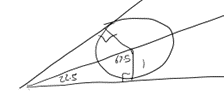
\includegraphics[width=0.25\linewidth]{images/t1w8q3_ans2.png}
    \end{figure}
    We can get an exact value now for the base of the triangle by using the tangent ratio.\\
    \(
    \theta=22.5\\
    \tan(2\theta)=\tan(45)\\
    \tan(2\theta)=1\\
    \frac{2\tan(\theta)}{1-\tan^2(\theta)}=1\\
    2\tan(\theta)=1-\tan^2(\theta)\\
    \tan^2(\theta)+2\tan(\theta)-1=0\\
    \tan(\theta)=\frac{-2+\sqrt{8}}{2}=-1+\sqrt{2}=\sqrt{2}-1\\
    \)
    (Disregard the negative solution as we know \(tan(18)\) is positive.)\\
    \begin{figure}[H]
        \centering
        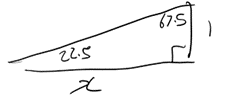
\includegraphics[width=0.25\linewidth]{images/t1w8q3_ans3.png}
    \end{figure}
    The tangent ratio is \(\frac{O}{H}\), which gives us:\\
    \(\sqrt{2}-1=\frac{1}{x}\)\\
    \(x=\frac{1}{\sqrt{2}-1}=\sqrt{2}+1\)\\

    So, we know that the base is \(\sqrt{2}+1\) times bigger than the radius.\\
    Using Pythagoras, we can also find an expression for the hypotenuse:\\
    \(h^2=1^2+(\sqrt{2}+1)^2\)\\
    \(h=\sqrt{4+2\sqrt{2}}\)\\
    \begin{figure}[H]
        \centering
        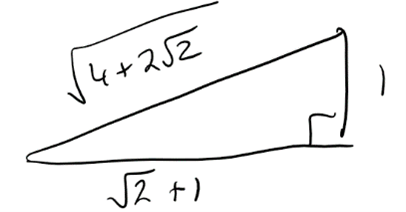
\includegraphics[width=0.25\linewidth]{images/t1w8q3_ans4.png}
    \end{figure}
    We can now draw a larger triangle out to the centre of the second circle (with radius R), and form an equation to find that radius. Note that the base of this triangle is \(\sqrt{2}+1\) times bigger than R as it is similar to the smaller triangle.
    \begin{figure}[H]
        \centering
        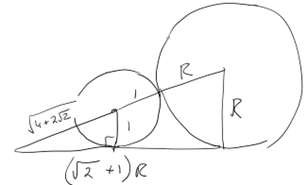
\includegraphics{images/t1w8q3_ans5.png}
    \end{figure}
    \(R^2+(\sqrt{2}+1)^2 R^2=(\sqrt{4+2\sqrt{2}}+1+R)^2\)\\
    
\((R^2+3R^2+2\sqrt{2})R^2=4+2\sqrt{2}+\sqrt{4+2\sqrt{2}}+R\sqrt{4+2\sqrt{2}}+\sqrt{4+2\sqrt{2}}+1+R+R\sqrt{4+2\sqrt{2}}+R+R^2
    \)\\
    
    \((3+2\sqrt{2})R^2-(2+2\sqrt{4+2\sqrt{2}})R-(2\sqrt{4+2\sqrt{2}}+2\sqrt{2}+5)=0\)\\
    
    Solving, R=2.24 (2dp).\\
    Since area = \(\pi r^2\), the larger circle is \(2.24^2=5.02\) times bigger.\\

    
\end{enumerate}

\end{document}